\chapter{Introduction}
\label{chp:1}
\section{Motivation}
\label{sec:1-motivation}
Alzheimer's disease (AD) is a complex neurological disorder
characterised by progressive structural brain damage and cognitive decline.
At present, AD remains incurable and difficult to treat,
placing a significant strain on those affected by the disease and society as a
whole. Despite the plentiful resources devoted to the treatment and
understanding of the diseases, the development of pharmacological interventions
has made little progress over the past several decades. Currently, research on
the aetiology of AD comprises investigation into numerous theories, including
the cholinergic hypothesis, the amyloid hypothesis and the prion-like
propagation hypothesis, among others \cite{liu2019history}. The failure to make
progress in designing effective disease altering treatments has motivated the
use of interdisciplinary investigation to help unify our knowledge of AD and
better understand its mechanisms. 

An important obstacle hindering scientific investigation of the processes
underlying Alzheimer's is the difficulty in making and understanding
observations of the disease in-vivo. It is challenging to make accurate
measurements of biological processes occurring over time in the human brain and
equally as difficult to interpret them. Over recent decades, increasingly
sophisticated technologies have been developed to image human brains, notably
positron emission tomography (PET) scanning and magnetic resonance imaging
(MRI). Brain imaging has facilitated scientists in building upon theories of AD
developed using in-vitro and in-vivo animal studies.  
In particular, neuroimaging studies have validated post-mortem studies into
protein staging \cite{Ossenkoppele2016,SCHOLL2016971,lowe2016, cho2016vivo},
patterns of atrophy \cite{jack2018nia,whitewell2010}, and changes to functional
activity \cite{chen2019functional}. Researchers have recognised the value of
these data and several open neuroimaging databases now exist to accelerate
investigation, including the Alzheimer's Disease Neuroimaging Initiative (ADNI),
the Human Connectome Project, the Swedish BioFINDER study and more, making
the process of obtaining and analysing observations less cumbersome. 

However, progress is still slow, in part because of the unyielding challenge of
modelling high dimensional neuroimaging data. This thesis aims to address this
problem through the marriage of dynamical systems and probabilistic inference.
The former allows for interpretability of high dimensional data through 
parsimonious mechanistic models; the latter
allows us to quantify the uncertainty present throughout the stages of such
modelling, from parameter identification and uncertainty to model selection. In
combination, these methods provide useful for investigation into AD by
diminishing obstacles of data interpretation. 

Interrogating AD in this way requires at least three components: biological
understanding, data, and models. Biological understanding is needed to formulate
theories and data is needed to test  
them. I will now briefly overview key features of \AB and \TP and current
methods used for making in-vivo observations in humans, before discussing the
modelling framework employed and the sources of uncertainty present.

\section{Biological Mechanisms of Alzheimer's Disease}
\label{sec:1-bio-ad}

% Several theories regarding the processes underlying AD development have been
% proposed and it continues to be an active research area. Theories include
% neurotransmitter dysfunction \cite{davies1976selective, francis1999cholinergic},
% protein aggregation
% \cite{selkoe1991molecular,hardy1991amyloid,walker2015neurodegenerative} and
% inhibited clearance of neurotoxins \cite{rasmussen2018glymphatic}. The main
% thrust of AD research in recent decades has focussed on the role of misfolded
% proteins, namely, Amyloid-$\beta$, \AB, which aggregate to form senile plaques, and
% $\tau$-protein, \TP, which aggregates into tangles
% \cite{jucker2013self,jucker2018propagation,walker2018standard}. In this section,
% I will briefly overview important results regarding these proteins and and their
% pathological mechanisms. 

A leading proposal for the the aetiology of AD is the prion-like propagation
hypothesis, which posits that pathology follows from prion-like processes of \AB
and \TP propagating and aggregating throughout the brain, causing tissue damage
and degeneration \cite{walker2015neurodegenerative, goedert2015alzheimer,
aoyagi2019abeta}. Early investigations focussed primarily on the role of \AB in
AD pathology \cite{selkoe1991molecular, hardy1991amyloid, hardy1992alzheimer,
hardy2002amyloid}, however, growing evidence suggests that both \AB and \TP are
necessary for AD pathology to \cite{selkoe2016amyloid, kametani2018reconsideration,
aoyagi2019abeta, ossenkoppele2022amyloid}.  

While \AB and \TP have different functions and properties, their toxic forms
both exhibit an ability to self-propagate by inducing conformational changes to
their healthy counterparts \cite{prusiner1991, prusiner1998,
walker2015neurodegenerative}. This prion-like property of templating begets the
ability of \AB and \TP to self-propagate. Their accumulation follows from at
least two processes: first, the aggregation of toxic \AB and \TP into senile 
plaques and tangles, respectively;
second, inhibited clearance of toxic aggregates
\cite{duyckaerts2009classification,tarasoff2015clearance}. An important part of 
modelling the evolution of \AB and \TP in the brain will rely on accurately 
describing the prion-like process.

\begin{figure}[t]
    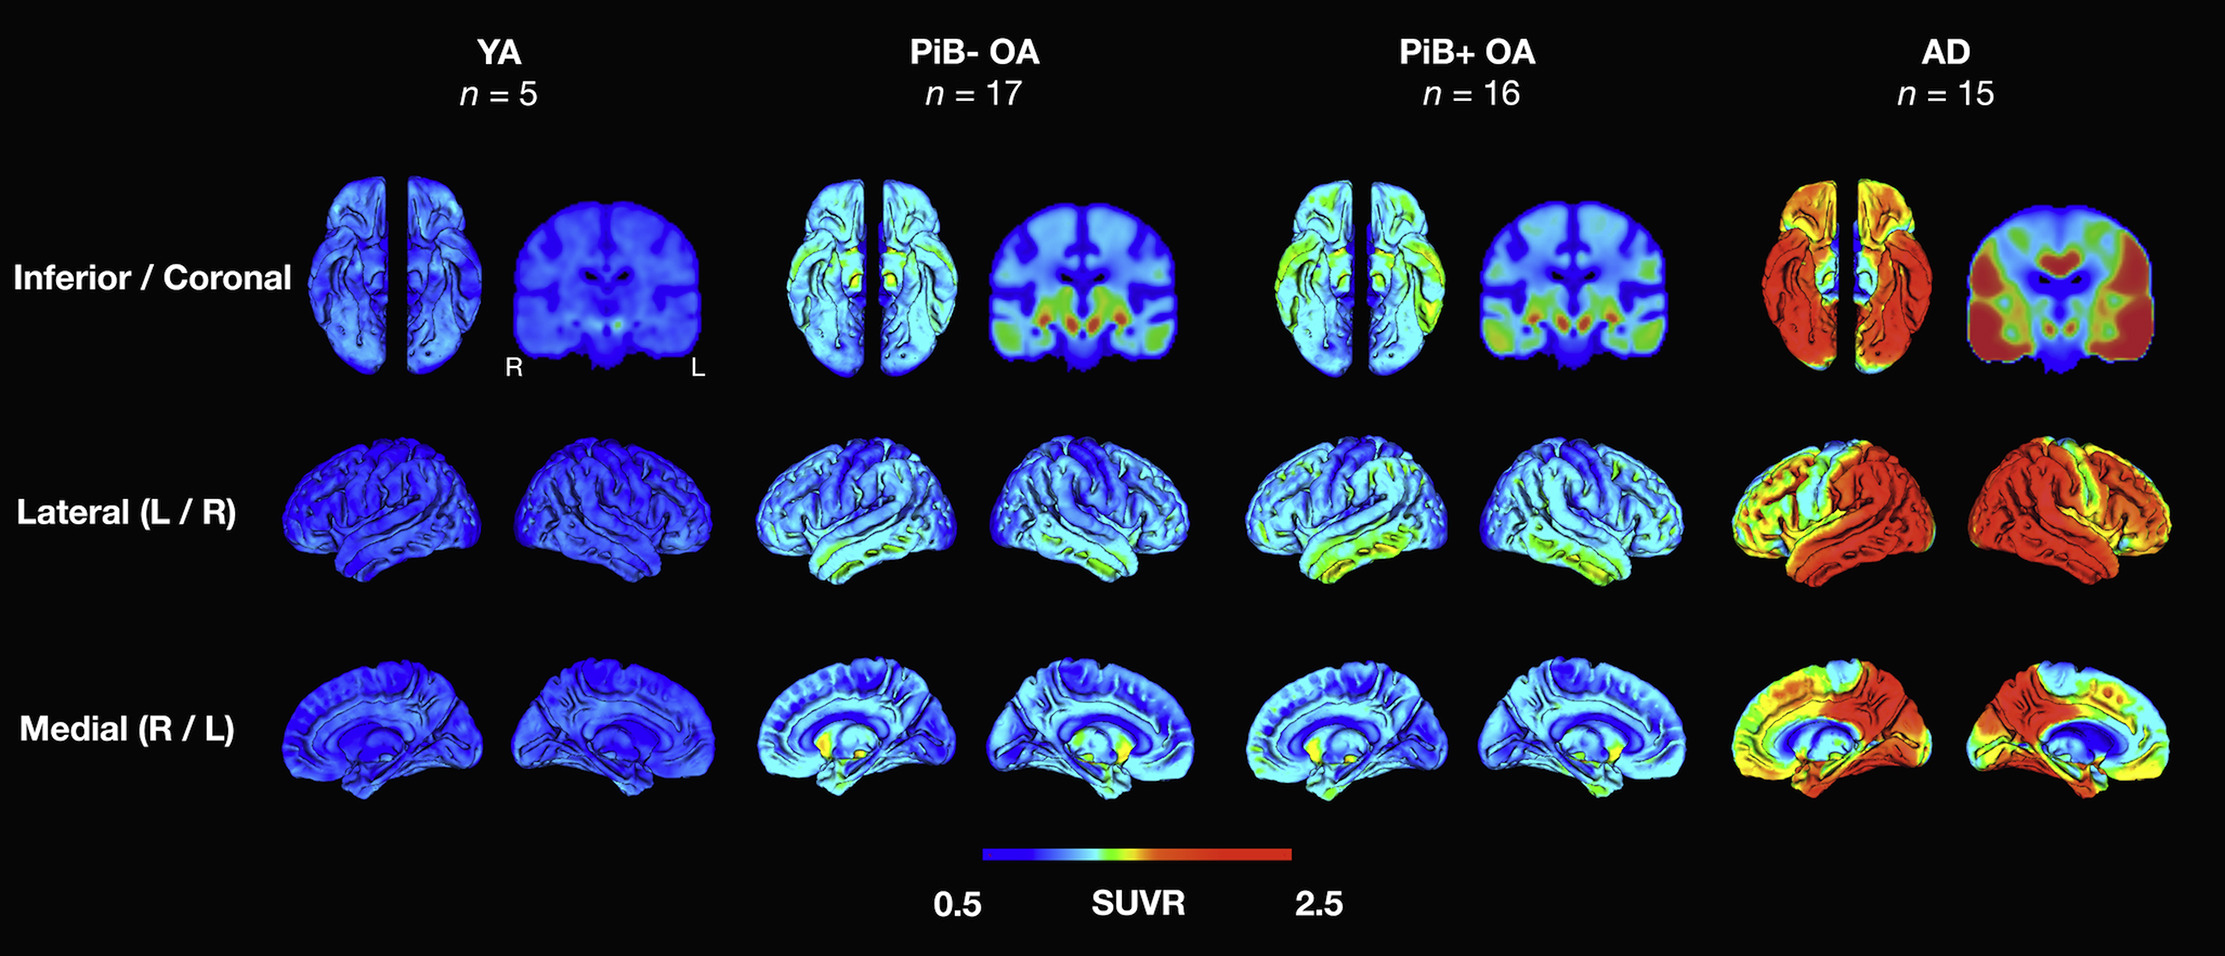
\includegraphics[width=\textwidth]{scholl-stages.jpeg}
    \centering
    \caption{\textbf{Stages of $\tau$-protein progression from SUVR.} 
    Figure adapted from \cite{SCHOLL2016971}, showing the mean \TP
    SUVR in a young adult population (YA), older adults (OA) with and without
    amyloid (determined by PiB PET), PiB- and PiB+, respectively, and subjects
    diagnosed with AD.}
    \label{fig:taustaging}
\end{figure}

In parallel with evidence toward the prion-like nature of \AB and \TP, AD
patients exhibit conserved patterns in the spread of these proteins through the
brain \cite{braak1991neuropathological, grothe2031, SCHOLL2016971,cho2016vivo}.
Typically, \AB begins globally in the neocortex and progresses subcortically.
Conversely and in a more pronounced fashion, whereas \TP displays more
incremental staging, starting from the entorhinal and spreading regions to
surrounding medial temporal structures, then the lateral temporal and then
finally into frontal and parietal cortices \cite{lowe2016,
SCHOLL2016971,Ossenkoppele2016, cho2016vivo}. The progression of atrophy is
correlated to the progression of toxic proteins, particularly with that of \TP
\cite{harrison2019longitudinal, xia2017association, cho2016vivo, jack2018nia,
pini2016}. The stereotypical patterns of toxic protein deposition and atrophy
provide a valuable bio-marker for the assessment AD pathology, particularly in
regions effected early in disease progression such as the hippocampus
\cite{echavarri2011atrophy, jack2011steps, eskildsen2015structural}.

\section{Imaging Alzheimer's Disease}\label{sec:1-imaging}

The ability to compare models and observations is crucial for determining their
utility. At present, observations are gathered through brain imaging,
namely PET studies and structural MRI (sMRI). There are a number of
publicly available data libraries containing such data specific to AD, most
notably the Alzheimer's Disease Neuroimaging Initiative (ADNI) and the Swedish
BioFINDER study. Additionally, there are a number of community standard software
libraries for the analysis of brain images. Particular software that are
utilised throughout the work presented here are FreeSurfer
\cite{fischl2012freesurfer} and FSL \cite{jenkinson2012fsl}. The combination of
publicly available data and analysis software has eased the burden on modellers
for finding and processing observational data.  

Since its inception, neuroimaging has proved a valuable tool for investigating
AD in humans. Without such methods, it would be near impossible to analyse
practically AD pathology in-vivo in human brains. The recent advent of \TP PET
tracers has allowed for such observations to be made
\cite{schwarz2016regional,xia201318f, marquie2015validating,
honer2018preclinical}. Two of the most popular radiotracers are the first
generation AV1451, used in ADNI \cite{landau2016flortaucipir}, and second
generation RO948 used in the second Swedish BioFINDER study (BF2)
\cite{ossenkoppele2021accuracy}. These tracers primarily bind to tau lesions
comprised of paired helical filaments, which allows for the quantification of
\TP related AD pathology \cite{smith2020head}. However, radiotracers also
exhibit off-target binding, attaching to molecules other than paired-helical
filaments of \TP and resulting in false signal. This can significantly limit the
utility of tracers in the affected brain regions. AV1451 signal exhibits
particularly strong contamination in the basal ganglia and choroid plexus
\cite{lowe2016autoradiographic,lemoine2018,choi2018off}. While these are not
areas that typically show particularly strong invasion in AD, the affect of
off-target binding interferers with signal in important surrounding areas,
namely the hippocampus \cite{johnson2016tau, lowe2016autoradiographic}. These
issues are partially circumvented with next generation tracers, such as RO498,
that show negligible binding in the choroid plexus and reduced binding the basal
ganglia \cite{smith2020head, kuwabara2018evaluation, wong2018characterization}. 

An example of how \TP PET can be used to monitor disease progression is shown in
\cref{fig:taustaging}, adapted from \cite{SCHOLL2016971}. Here, the authors use
a combination of an \AB PET tracer (PiB) and a \TP tracer (AV1451) to track
disease progression from young adults (YA), to older adults without \AB (PiB-
OA), older adults with \AB (PiB+ OA) and finally patients diagnosed with AD.
\cref{fig:taustaging} shows the mean \TP PET standardised uptake value ratio
(SUVR) in each of these groups. The figure demonstrates two important features
of \TP PET. First, \TP PET is able to capture the pronounced staging of \TP
through the brain during AD progression. Second, \TP staging observed through
PET differs from that observed through post-mortem histological analysis
\cite{braak1991neuropathological}, in particular through strong \TP signal
involvement in the occipital lobe. The differences in staging likely arise from
regional variations in tracer dynamics, such as uptake and binding affinity.
Tracer staging profiles have now been extensively validated \cite{lowe2016,
cho2016vivo, vogel2020spread, biel2021tau, vogel2021four}.

These data have been used extensively by modellers for parameter calibration and
validation \cite{vogel2020spread,schafer2020network,schafer2021bayesian}.
Similarly, studies using structural MRI have shown how atrophy progresses during
AD \cite{whitewell2010}, highlighting the relationship between atrophy and \TP,
but not \AB \cite{Ossenkoppele2016,SCHOLL2016971,lowe2016}. As yet, few studies,
have used structural MRI as observations to fit models, however, their relative
abundance compared to PET data make them a valuable resource for modelling,
especially if they can be usefully combined for multimodal inference
\cite{raj2012network,raj2015network,schafer2022correlating}. Overall,
neuroimaging has provided a wealth of knowledge and data that has advanced AD
research in its own right, and has also facilitated modelling studies probing
disease mechanism.

\section{Dynamical Models of AD}\label{sec:1-uncertainty}

Network models of neurodegeneration have been used extensively to study the
progression of toxic proteins during AD but come with a number of challenges,
some inherent with dynamical systems models and some particular to the modelling
domain, i.e. network neuroscience.  The basic mechanisms these models describe
are transport across axons and growth via an autocatalytic prion-like process.
The first model, describing only transport through axons, was provided by
\cite{raj2012network} and laid the foundation for other groups to expand on this
with more expressive models that describe growth
\cite{fornari2019prion,fornari2020spatially,weickenmeier2018multiphysics}.  
The general form of these models is a system of ordinary differential equations
on a graph: 
\begin{equation}\label{equ:general-system}
\odl{\mathbf{u}}{t} = \tns{f}(\tns{u},  t; \tns{p}, \tns{L}),
\end{equation}
where $\tns{f}$ is a vector valued function in time, with state vector $\tns{u}
\in \mathbb{R}^N$, additionally depending on parameters, $\tns{p} \in
\mathbb{R}^p$, and a $N \times N$ Laplacian matrix, $\tns{L}$, derived from a
graph used to define the domain of the system. Representing the system in this
way highlights the challenges present in the modelling process, since each
element of the system brings its own form of uncertainty that requires
quantification and rectification. 

First, there is uncertainty about the nature of the function $\tns{f}$,
principally due to our limited understanding of AD pathology. Several models
have been presented in the literature, including the simple network diffusion
model \cite{raj2012network,raj2015network}, the epidemic spreading model
\cite{vogel2020spread} and a host of reaction-diffusion equations
\cite{fornari2019prion,fornari2020spatially}. Each of these models imbue
different processes and assumptions into a model of AD pathology and at present
there is little evidence to choose one over another. Thus it is important to  be
able to identify which of these models is most appropriate given the available
data. There are numerous methods available for this, including a host of
information criteria, such as the Akaike information criteria, and more advanced
methods such as Bayesian leave-one-out cross validation
\cite{gelman2014understanding}.

\begin{figure}[t]
    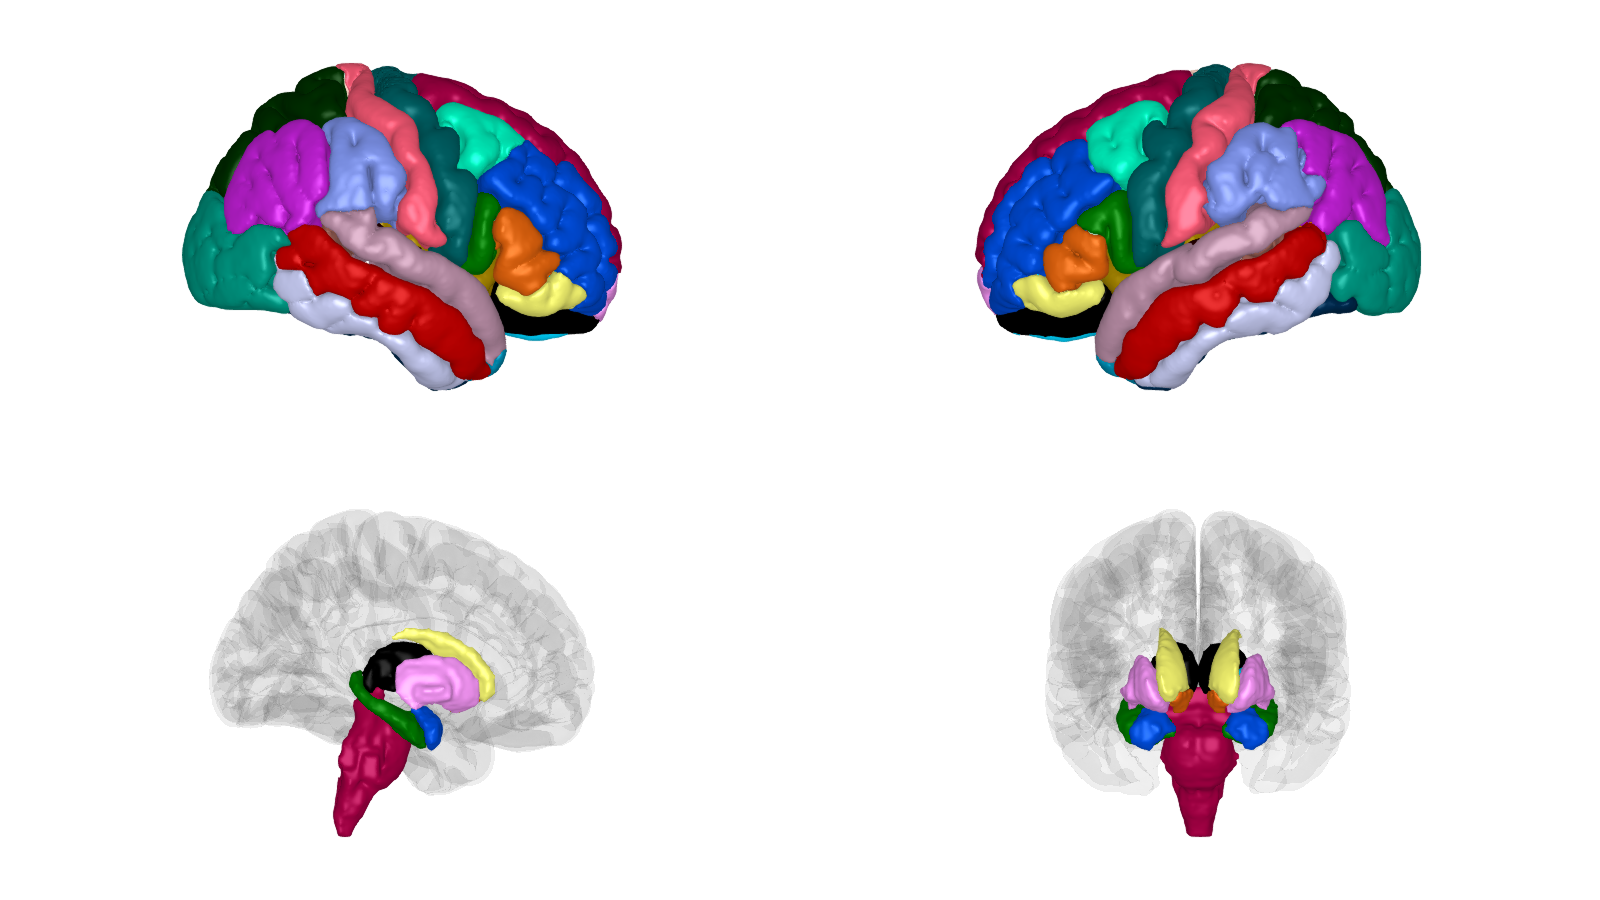
\includegraphics[width=15cm, height=9cm]{parcellation.png}
    \centering
    \caption{\textbf{The DKT parcellation}. The standard FreeSurfer DKT
    parcellation shown on a MNI brain. Top: 68 cortical regions for left and
    right hemispheres. Bottom: 15 subcortical regions, including the brainstem}
    \label{fig:parcellation}
\end{figure}

Second, there is considerable uncertainty associated with the graph used to
define the dynamical system. The graph not only defines the state vector,
$\tns{u}$, but the transport between its elements, and therefore its properties
can have a large effect on the dynamics of the system. The process of
generating a graph, referred to in network neuroscience as a connectome, can be
broadly separated into two processes: 1) parcellating the brain; 2) performing
tractography. Each of these two processes are active areas of research in
imaging neuroscience and there is no canonical choice for either, leading to
sources of uncertainty stemming from both. 

For the current work, we generate connectomes using the
Desikan-Killiany-Tourville (DKT) parcellation supplied as standard in the FreeSurfer
software package \cite{fischl2004automatically, klein2012101} and visualised in
\cref{fig:parcellation}. However, there are many alternative parcellation
choices, each of which characterise different features of brain, e.g. anatomy,
functional connectivity, size of regions, gyrification, among others
\cite{lawrence2021standardizing, moghimi2021review}. It is not yet known whether
some parcellations are better suited than others for marco-scale connectome
modelling.  

Tractography is a process of reconstructing the neuronal connections between
brain regions from diffusion weighted MRI imaging (dMRI). There are two broad
families of tractography methods, deterministic and probabilistic. Both methods
seek to simulate streamlines, synthetic fibers that follow the estimated fiber
orientation at each voxel. Deterministic tractography follows the trajectory of
streamlines using fixed fiber orientations at each voxel, whereas probabilistic
tractography uses a distribution of fiber orientations at each voxel to account
for uncertainty in possible streamline direction \cite{sarwar2019mapping}. The
output of tractography is an adjacency matrix that defines a graph representing
connections between regions of a given parcellation. Connectomes generated using
different procedures are shown in \cref{fig:connectome}.
\cref{fig:connectome-diffusive-fsl} shows a connectome generated with
probabilistic tractography using FSL, while \cref{fig:connectome-diffusive-pit}
shows one generated using deterministic tractography
\cite{szalkai2017parameterizable,kerepesi2017braingraph}, distributed by the PIT
group through \url{www.braingraph.org}. Differences in network topology, such as
those shown between
\cref{fig:connectome-diffusive-fsl,fig:connectome-diffusive-pit}, can have
significant effects on the dynamics exhibited on those networks
\cite{putra2021braiding}. Together with the lack of consensus about how to
generate connectomes, this creates a large source of uncertainty in the
modelling process. In this work, we use connectomes generated using the default
pipelines in FSL, which have been extensively validated
\cite{behrens2003characterization,behrens2007probabilistic,warrington2020xtract},
and data from the HCP.
\begin{figure}[t]
    \centering
    \begin{subfigure}[b]{0.8\textwidth}
        \centering
        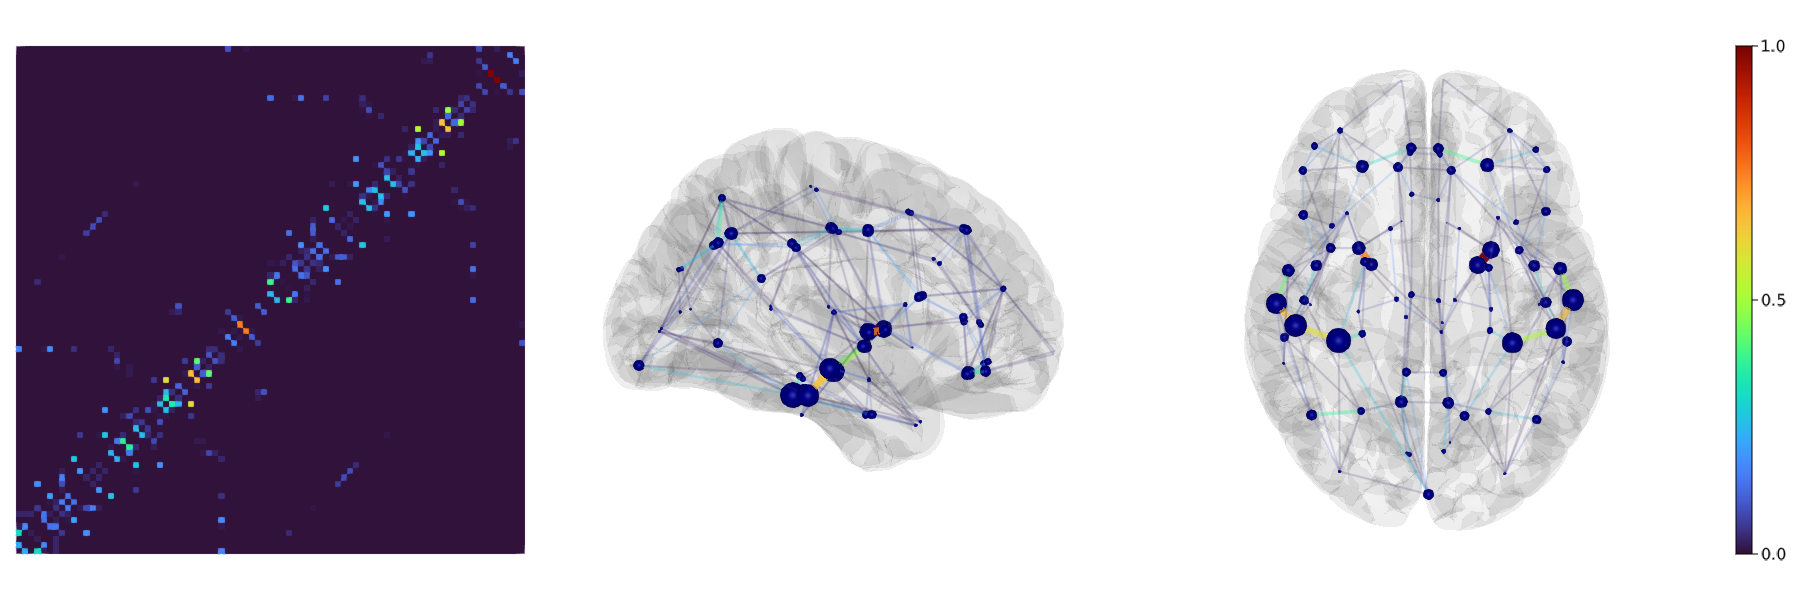
\includegraphics[width=\textwidth]{connectomes/connectome-diffusive.png}
        \caption{Probabilistic connectome with diffusive weights}
        \label{fig:connectome-diffusive-fsl}
    \end{subfigure}
    \begin{subfigure}[b]{0.8\textwidth}
        \centering
        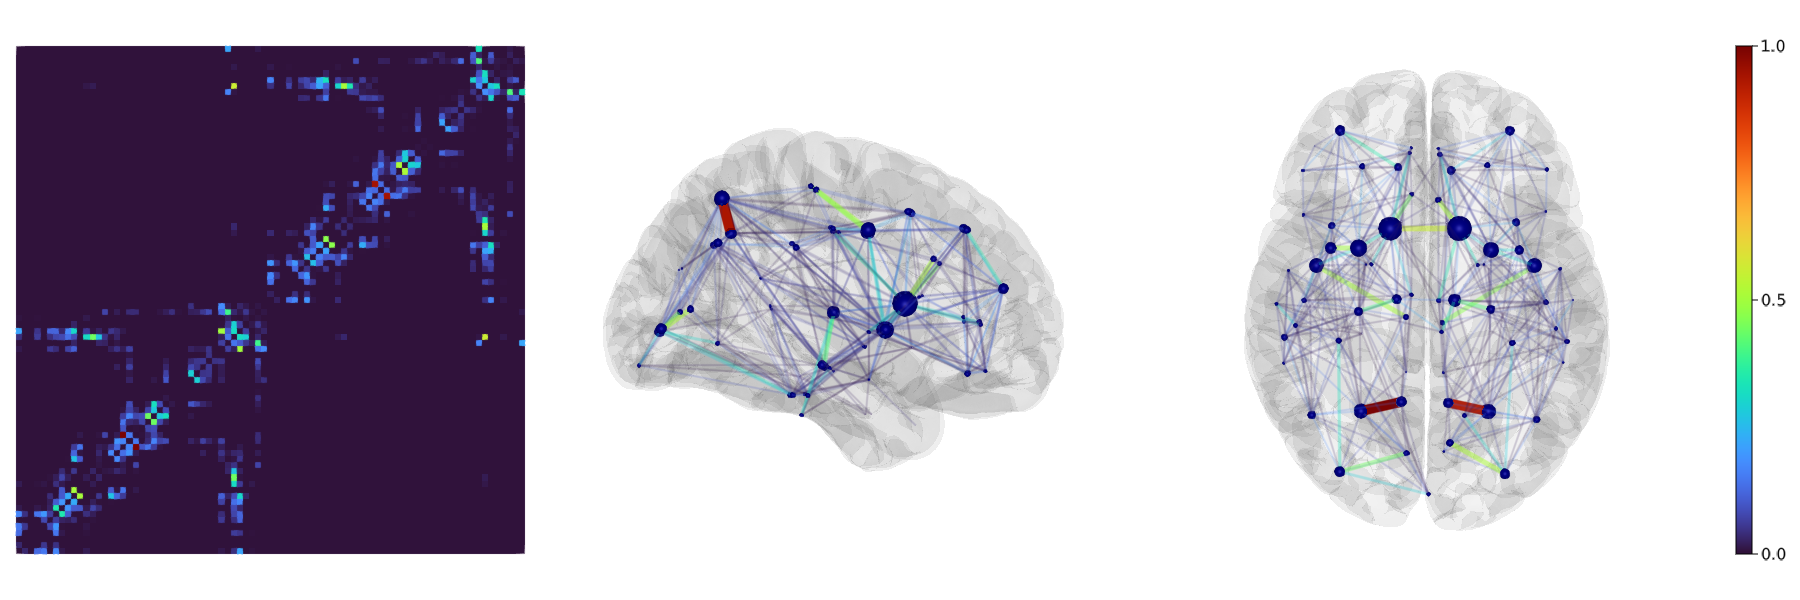
\includegraphics[width=\textwidth]{connectomes/connectome-pit.png}
        \caption{Deterministic connectome with diffusive weights}
        \label{fig:connectome-diffusive-pit}
    \end{subfigure}
    \caption{\textbf{Connectomes made with different tractography procedures}.\\
    Both connectomes are made using the DKT atlas to define regions of interest.
    Left: Shown are weighted adjacency matrices normalised to the maximum
    values. Right: networks visualised on the brain; edges coloured by weight
    and and vertices sized by degree. Networks have been filtered using a naive
    threshold of 0.01. \textbf{(a)} Made using FSL probabilistic tractography
    \cite{behrens2003characterization,behrens2007probabilistic}. \textbf{(b)}
    Made using MRtrix deterministic tractography and distributed by the PIT
    group through \url{www.braingraph.org} \cite{kerepesi2017braingraph}.}
       \label{fig:connectome}
\end{figure}

Third, there is parametric uncertainty associated with the parameter vector,
$\mathbf{p}$. For any given dynamical system, variations in parameters can lead
to different model behaviours. In general, it is difficult to infer from
observations alone the parameters of the dynamical system, a problem that is
made more challenging in the presence of observation noise. Popular methods for
inferring parameter values include least squares regression, maximum likelihood
estimation and maximum a-posteriori estimation and have been used in the network
neurodegeneration literature for model validation
\cite{raj2012network,raj2015network,vogel2020spread}. However, forr ill-posed
problems with sparse and noisy observations, and where data are assumed to be
generated from a non-linear process, these methods are unsuitable since they do
not account for potentially significant parametric uncertainty. The effect of
parameter variations on the dynamics of models for neurodegeneration has been
shown in \cite{putra2021braiding}. We have recently presented work which has
incorporated Bayesian analysis into the validation pipeline, which allows for
the quantification of uncertainty
\cite{schafer2020network,schafer2021bayesian,schafer2022correlating}. The
results highlight that there can be considerable variation in parameters between
individuals and groups for a given set of observations. A framework for handling
sources of uncertainty has been the focus of this project thus far and will be
discussed in \cref{chp:2}, with applications in \cref{chp:3}. 

\section{Research Aims and Report Overview}

\subsection{Research Aims}
My aim is to establish a mathematical and software framework for validating
dynamical models of AD with human neuroimaging data. My objectives are to: 

\begin{enumerate} 
    \item Develop a unified mathematical and software pipeline that
    simplifies dynamical modelling of AD and inference with patient data. 
    \item Apply this framework to answer specific questions about AD
    progression.
\end{enumerate}

\subsection{Report Overview}
The remainder of the report is organised as follows. In \cref{chp:2}, I
will discuss the mathematical models that are used throughout this report. I
will also overview the general problem of using Bayesian inference for
time-series problems. In \cref{chp:3}, I will present recent work on the
application of dynamical systems, generative modelling and Bayesian inference to
problems in neurodegeneration. In \cref{chp:4}, I offer some concluding
remarks and a proposal for future work.
Parts of this report are taken from the following publications and highlighted
accordingly: 
\begin{itemize}
    \item \fullcite{schafer2022correlating} \textbf{Joint first author.}
    \item \fullcite{schafer2021predicting} \textbf{Joint first author.}
    \item \fullcite{putra2021braiding}
    \item \fullcite{thompson2020}
\end{itemize}
The results presented in \cref{chp:3} reflects my most recent work 
and is currently being prepared for publication.

